
C++20對現有的併發性進行了增強,但我們將重點關注新添加的特性:協程。協程具有中斷和恢復功能的線程,在幾種主要的應用程序中很有用。可以極大地簡化事件驅動程序的編寫,對於竊取工作的線程池來說,那必然要使用協程,而且會讓異步I/O和其他異步的代碼更加簡單

\subsubsubsection{8.4.1\hspace{0.2cm}介紹協程}

協同程序有兩種風格:\textbf{有棧}和\textbf{無棧}。有棧協程有時也稱為\textbf{纖程}(fiber),類似於在堆棧上分配狀態的函數。無棧協程沒有相應的堆棧,狀態存儲在堆中。有棧協程更加強大和靈活,但是無棧協程會更高效。

本書中,因為C++20支持,將重點關注無棧協程。這是一個不尋常的概念,在展示C++特有的語法和示例之前,先來瞭解一下。

常規的C++函數總有一個相應的堆棧框架。只要函數在運行,棧幀就存在,所有的局部變量和其他狀態都存儲在這裡。下面是一個簡單的函數\texttt{f()}:

\begin{lstlisting}[style=styleCXX]
void f() {
	…
}
\end{lstlisting}

其中有一個棧幀。再函數\texttt{f()}調用另一個函數\texttt{g()}時:

\begin{lstlisting}[style=styleCXX]
void g() {
	…
}
void f() {
	…
	g();
	…
}
\end{lstlisting}

函數\texttt{g()}在函數運行時也有一個棧幀。 

參考下圖:

%\hspace*{\fill} \\ %插入空行
\begin{center}
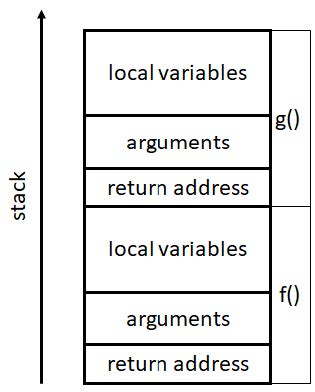
\includegraphics[width=0.5\textwidth]{content/2/chapter8/images/5.jpg}\\
圖8.5 - 常規函數的棧幀
\end{center}

當函數\texttt{g()}退出時,它的棧幀會銷燬,只有函數\texttt{f()}的棧幀保留了下來。

無棧協程的狀存儲在堆上,這種分配稱為\textbf{活幀}。活幀與協程句柄相關聯,協程句柄是一個智能指針的對象。可以發出和返回函數的調用,只要句柄沒有損壞,活幀就一直存在。

協程還需要堆棧空間,調用其他函數。該空間在調用者的堆棧上分配,下面展示其工作原理(C++語法有所不同,所以現在把協程相關的行為想象成偽代碼):

\begin{lstlisting}[style=styleCXX]
void g() {
	…
}
void coro() { // coroutine
	…
	g();
	…
}
void f() {
	…
	std::coroutine_handle<???> H; // Not the real syntax
	coro();
	…
}
\end{lstlisting}

對應的內存分配如下圖所示:

%\hspace*{\fill} \\ %插入空行
\begin{center}
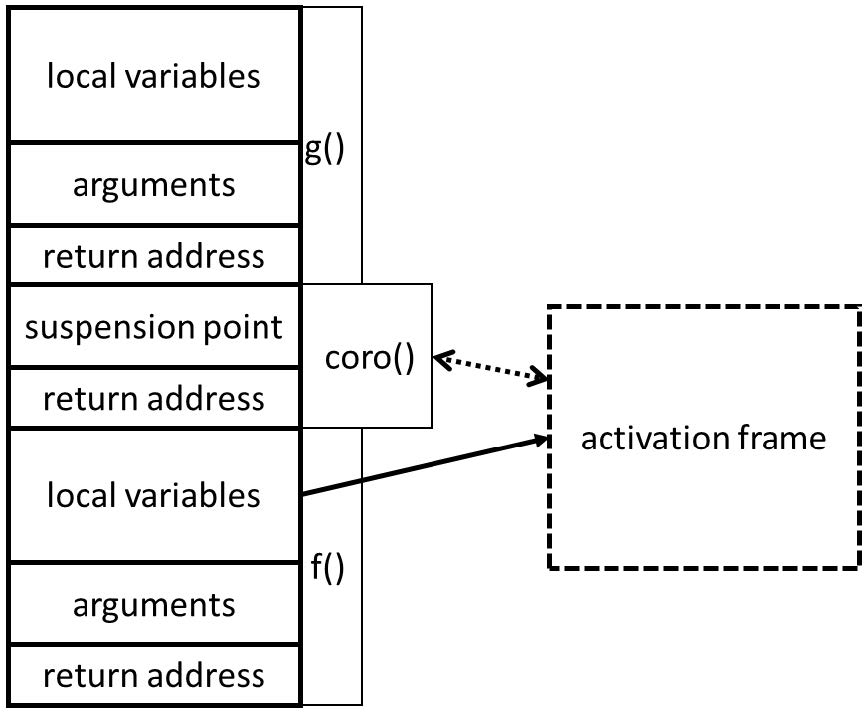
\includegraphics[width=0.6\textwidth]{content/2/chapter8/images/6.jpg}\\
圖8.6 - 調用協程
\end{center}

函數\texttt{f()}創建協程句柄,擁有活幀。然後調用協程函數\texttt{coro()}。這時有堆棧分配,協程在堆棧上存儲了在掛起時返回的地址(記住,協程是可以掛起自己的函數)。協程可以調用另一個函數\texttt{g()},將\texttt{g()}的棧幀分配到堆棧上。此時,協程不能再掛起,只有協程頂層函數可以掛起。函數\texttt{g()}無論誰調用最終都會返回,以同樣的方式運行,這將破壞它的棧幀。協程現在可以掛起自己,所以假設它掛起了。 

這是有棧協程和無棧協程的關鍵區別。有棧協程可以在函數調用的任意深度處掛起,並從那裡恢復。但是這種靈活性需要很高的內存成本,尤其是運行時成本。無棧協程由於其有限的狀態,效率要高很多。

當協程掛起時,恢復協程所需的部分狀態會存儲在活幀中。然後銷燬協程的棧幀,並將控制權返回給調用者,直至協程調用的位置。如果協程完成,也會發生同樣的情況,但是調用者有一種方法可以查詢協程的狀態是掛起還是完成。

調用者繼續執行他的操作,並可以使用其他函數:

\begin{lstlisting}[style=styleCXX]
void h() {
	…
}
void coro() {…} // coroutine
void f() {
	…
	std::coroutine_handle<???> H; // Not the real syntax
	coro();
	h(); // Called after coro() is suspended
	…
}
\end{lstlisting}

內存分配看起來如下所示:

%\hspace*{\fill} \\ %插入空行
\begin{center}
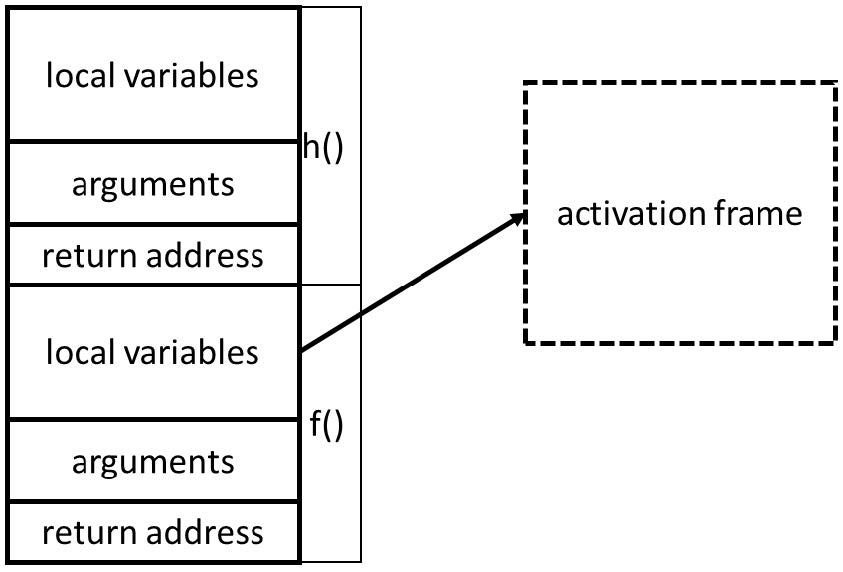
\includegraphics[width=0.6\textwidth]{content/2/chapter8/images/7.jpg}\\
圖8.7 - 掛起協程,繼續執行
\end{center}

注意,沒有與協程對應的棧幀,只有堆分配的活幀。只要句柄對象處於活動狀態,協程就可以恢復。不一定是調用和恢復協程的同一函數,例如:如果句柄可用,函數\texttt{h()}就可以恢復:

\begin{lstlisting}[style=styleCXX]
void h(H) {
	H.resume(); // Not the real syntax
}
void coro() {…} // coroutine
void f() {
	…
	std::coroutine_handle<???> H; // Not the real syntax
	coro();
	 h(H); // Called after coro() is suspended
	…
}
\end{lstlisting}

協程從暫停的地方重新開始,狀態從活幀中恢復(堆棧分配將像往常一樣):

%\hspace*{\fill} \\ %插入空行
\begin{center}
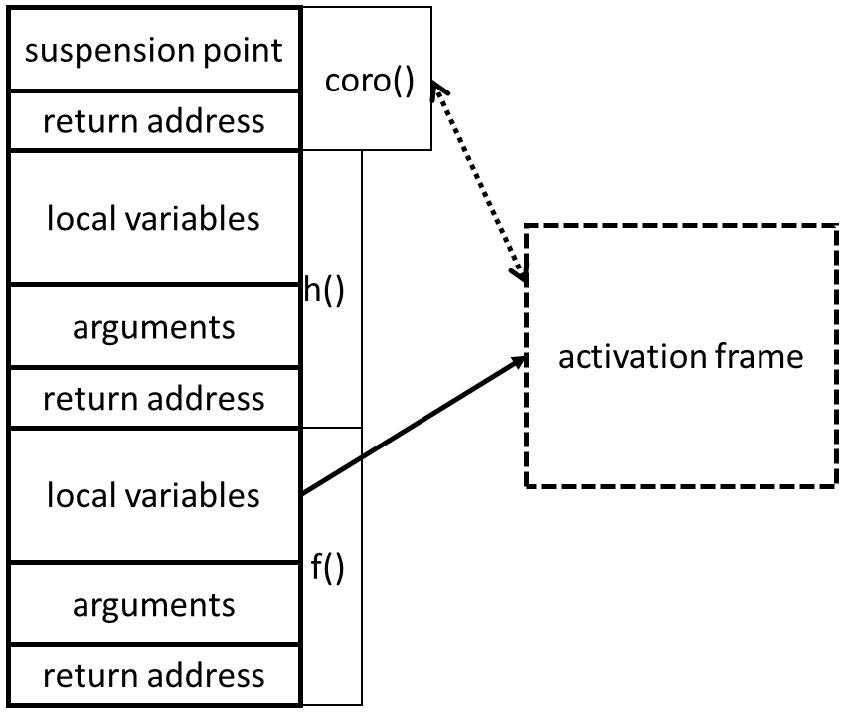
\includegraphics[width=0.6\textwidth]{content/2/chapter8/images/8.jpg}\\
圖8.8 - 協程從不同的函數處恢復
\end{center}.

最終,協程完成,句柄銷燬。這將釋放與協程關聯的所有內存。

以下是關於C++20協程需要了解的主要內容:

\begin{itemize}
\item
協程是可以掛起自己的函數。這與操作系統掛起一個線程不同,掛起一個協程是由開發者顯式地完成的(多任務協作)。

\item
與棧幀相關聯的常規函數不同,協程具有句柄對象。只要句柄處於活動狀態,協程狀態就會保持。

\item
協程掛起後,控制權將返回給調用者,調用者可以繼續以相同的方式運行,就像協程已經完成一樣。 

\item 
協程可以從任何位置恢復,不一定是調用者本身。此外,協程甚至可以從不同的線程恢復(將在本節後面看到一個示例)。協程從掛起點恢復,並繼續運行,就像什麼都沒發生一樣(但可能在不同的線程上運行)。
\end{itemize}

\subsubsubsection{8.4.2\hspace{0.2cm}C++的協程}

現在看一下C++語言的構造,這些構造可用於協程編程。 

首先,需要一個支持該特性的編譯器。GCC和Clang在他們的最新版本中都支持協程,但不幸的是,方式不同。對於GCC您需要版本11或更高版本。對於Clang,在版本10中添加了部分支持,並在以後的版本中進行了加強,但仍然是“實驗性的”。

首先,為了編譯協程代碼,需要在命令行上有一個編譯器選項(使用\texttt{-std=c++20}選項啟用C++20還不夠)。對於GCC,這個選項是\texttt{-fcoroutines}。對於Clang,選項是\texttt{-stdlib=libc++ -fcoroutines-ts}。最新版的Visual Studio只需要\texttt{/std:c++20}。

然後,需要包含協程頭文件。在GCC和Visual Studio中(根據標準),頭文件是\texttt{\#include <coroutine>},聲明的所有類都在標準命名空間\texttt{std}中。但在Clang中,頭文件是\texttt{\#include <experimental/coroutine>},使用的命名空間是\texttt{std::experimental}。

聲明協程不需要特殊的語法,協程只是普通的C++函數。使它們成為協程的是使用暫停操作\texttt{co\_await}或其\texttt{co\_yield}。然而,在函數體中調用這些操作是不夠的,C++中的協程對其返回類型有嚴格的要求。標準庫在聲明這些返回類型和其他處理協程所需的類時,沒有提供任何幫助。語言僅提供了一個使用協程進行編程的框架。因此,直接使用C++20協程代碼會非常冗長、重複,並且包含大量樣板代碼。實際中,每個使用協程的開發者都會使用一個可用的協程庫。 

實際編程中,也應該這樣做。本書中,將展示用簡單的C++編寫的示例。這樣做的目的是,不想引入任何特定的庫,而且這樣做會模糊讀者對實際情況的理解。對協程的支持是最近才出現的,這些庫也在迅速發展,現在選擇的庫不一定會一直好用。我們希望在C++的級別理解協程代碼,而不是在某個特定庫所呈現的抽象級別理解協程代碼。然後,應該根據自己的需要選擇一個庫,並使用抽象語法進行編程。

對與協程相關語法結構的全面描述非常不直觀。它是一個框架,而不是一個庫。出於這個原因,將使用示例來完成餘下的演示。如果真的想知道協程的所有語法要求,必須查找最新的出版物(或閱讀標準)進行了解。但是這些例子應該能對協程的功能有足夠的展示,也可以閱讀相關協程庫的文檔,並在程序中使用這個協程庫。

\subsubsubsection{8.4.3\hspace{0.2cm}協程用例}

第一個例子是C++中協程最常見的用法(標準為協程提供了一些顯式設計的語法),將實現一個惰性生成器。生成器是生成數據序列的函數。每次調用生成器,都會得到序列的一個新元素。惰性生成器是按需計算元素的生成器。

下面是一個基於C++20協程的惰性生成器:

\hspace*{\fill} \\ %插入空行
\noindent
\textbf{coroutines\_generator1.C}
\begin{lstlisting}[style=styleCXX]
generator<int> coro(){
	for (int i = 0;; ++i) {
		co_yield i;
	}
}
int main() {
	auto h = coro().h_;
	auto& promise = h.promise();
	for (int i = 0; i < 3; ++i) {
		std::cout << "counter: " << promise.value_ << 
		std::endl;
		h();
	}
	h.destroy();
}
\end{lstlisting}

這是底層的C++代碼,可以對其中涉及的每一步進行解釋。首先,協程\texttt{coro()}看起來像個函數,\texttt{co\_yield}操作符除外。此操作符掛起協程,並將值\texttt{i}返回給調用者。因為協程掛起,而不是終止,所以操作符可以執行多次。和其他函數一樣,協程在控件到達右大括號時終止。此時,無法恢復。通過\texttt{co\_return}(不應該使用常規的\texttt{return}),可以退出協程。

其次,協程的返回類型——生成器——需要定義的一種特殊類型,由於使用有很多要求,會導致了冗長的樣板代碼(任何協程庫都預定義了這樣的類型)。生成器包含一個嵌套的數據成員\texttt{h\_},而這就是協程句柄。隨著這個句柄的創建也會創建活幀。句柄與\texttt{promise}對象關聯,這與C++11的\texttt{std::promise}沒有任何關係。事實上,它根本不是標準類型之一,必須根據標準中列出的一組規則來定義它。執行結束時,句柄會銷燬,這也會銷燬協程的狀態。因此,句柄類似於指針。

最後,句柄是一個可調用對象。調用會恢復協程,因為\texttt{co\_yield}操作符在循環中,所以協程會生成下一個值,並立即再次掛起自己。 

通過為協程定義適當的返回類型,所有這些都可以奇妙地結合在一起。就像STL算法一樣,整個系統都受到規則的約束,這個過程中涉及到的所有類型都有期望。若這些期望沒有得到滿足,就無法編譯。現在來看看生成器的類型:

\begin{lstlisting}[style=styleCXX]
template <typename T> struct generator {
	struct promise_type {
		T value_ = -1;
		generator get_return_object() {
			using handle= std::coroutine_handle<promise_type>;
			return generator{handle::from_promise(*this)};
		}
		std::suspend_never initial_suspend() { return {}; }
		std::suspend_never final_suspend() noexcept { return 
			{}; }
		void unhandled_exception() {}
		std::suspend_always yield_value(T value) {
			value_ = value;
			return {};
		}
	};
	std::coroutine_handle<promise_type> h_;
};
\end{lstlisting}

首先,返回類型不必從模板生成,可以聲明一個整數生成器。通常,是對生成序列中的元素類型參數化的模板。其次,命名生成器沒有任何特殊之處,可以隨意調用該類型(大多數庫都提供了類似的模板,並將其稱為生成器)。另一方面,嵌套類型\texttt{generator::promise\_type}必須稱其為\texttt{promise\_type}。否則,程序將無法編譯。嵌套類型可以命名成其他類型,並在使用時,使用類型別名:

\begin{lstlisting}[style=styleCXX]
template <typename T> struct generator {
	struct promise { … };
	using promise_type = promise;
};
\end{lstlisting}

\texttt{promise\_type}類型\textit{必須}是\texttt{generator}類的嵌套類型(或者,協程返回的類型)。但是\texttt{promise}類不強制是嵌套類。通常是嵌套類,但可以在外部進行聲明。 

這裡需要\texttt{promise}類型的成員函數集合,包括簽名。注意,有些成員函數是\texttt{noexcept}的。這也是需求的一部分,若忽略此規範,程序將無法編譯。當然,即使函數不會拋出異常,也沒必要將其聲明為\texttt{noexcept}。 

對於不同的生成器,這些必需的函數實現可能更加複雜。這裡簡要描述他們的工作。

第一個非空函數\texttt{get\_return\_object()}是樣板代碼的一部分,看起來和前面的那個完全一樣,這個函數從句柄構造了一個新的生成器,而句柄又是由\texttt{promise}對象構造的,編譯器使用它獲得協程的結果。 

第二個非空函數\texttt{yield\_value()},在每次使用操作符\texttt{co\_yield}時調用,它的參數是\texttt{co\_yield}值。將值存儲在\texttt{promise}對象中,是協程將結果傳遞給調用者的常用方式。 

編譯器在第一次遇到\texttt{co\_yield}時調用\texttt{initial\_suspend()}。\texttt{final\_suspend()}在協程通過\texttt{co\_return}生成最後一個結果後調用,之後不能暫停。如果協程結束時沒有返回\texttt{co\_return},則調用\texttt{return\_void()}。最後,如果協同程序拋出了一個從其主體中逃逸的異常,則調用\texttt{unhandled\_exception()}。儘管些情況很罕見,使用者可以定製這些方法來處理其中每一種情況。

現在來看看它們是如何結合在一起,從而提供一個惰性生成器的。首先,創建協程句柄。在示例中,不保留生成器對象,只保留句柄。這不是必需的,可以保留生成器對象,並在其析構函數中銷燬句柄。協程一直運行,直到\texttt{co\_yield}掛起自己,控制權返回給調用者,而\texttt{co\_yield}的返回值在\texttt{promise}中捕獲。調用程序獲取此值,並通過調用該句柄恢復協程。協程從它掛起開始,一直運行到下一個\texttt{co\_yield}。 

生成器可以永遠運行(或者達到平臺上的最大整數值),流程永遠不會結束。如果需要一個有限長度的序列,可以執行\texttt{co\_return},或在流程結束後退出循環。參考以下代碼:

\begin{lstlisting}[style=styleCXX]
generator<int> coro(){
	for (int i = 0; i < 10; ++i) {
		co_yield i;
	}
}
\end{lstlisting}

現在有一個10個元素的序列。嘗試恢復協程之前,調用者必須檢查句柄成員函數\texttt{done()}的結果。

可以從代碼中的任何地方恢復協程(當然是在它掛起後),甚至可以從不同的線程恢復。這種情況下,協程開始在一個線程上執行和掛起,然後在另一個線程上運行它的其餘代碼。看一個例子:

\hspace*{\fill} \\ %插入空行
\noindent
\textbf{coroutines\_change\_threads.C}
\begin{lstlisting}[style=styleCXX]
task coro(std::jthread& t) {
	std::cout << "Coroutine started on thread: " <<
		std::this_thread::get_id() << '\n';
	co_await awaitable{t};
    std::cout << "Coroutine resumed on thread: " <<
		std::this_thread::get_id() << '\n';
	std::cout << "Coroutine done on thread: " <<
		std::this_thread::get_id() << '\n';
}
int main() {
	std::cout << "Main thread: " <<
		std::this_thread::get_id() << '\n';
	std::jthread t;
	coro(t);
	std::cout << "Main thread done: " << 
		std::this_thread::get_id() << std::endl;
}
\end{lstlisting}

先了解一些細節信息:\texttt{std::jthread}在C++20中添加,它只是一個可匯入的線程——它會連接到對象的析構函數中(幾乎所有使用線程的人都為此編寫了一個類,但現在有了一個標準的類)。現在可以來看看協程。 

瞭解一下協程的返回類型:

\begin{lstlisting}[style=styleCXX]
struct task{
	struct promise_type {
		task get_return_object() { return {}; }
		std::suspend_never initial_suspend() { return {}; }
		std::suspend_never final_suspend() noexcept { return 
			{}; }
		void return_void() {}
		void unhandled_exception() {}
	};
};
\end{lstlisting}

這可能是協程的最小返回類型。包含所有必需的樣板,而不包含其他內容。具體來說,返回類型是一個嵌套類型\texttt{promise\_type}類。該嵌套類型必須定義幾個成員函數,如下面的代碼所示。前面示例中的生成器類型包含這些內容,以及用於將結果返回給調用者的數據。當然,任務也可以根據需要具有內部狀態。

與前面的例子相比,第二個變化是任務掛起的方式。使用\texttt{co\_await},而不是\texttt{co\_yield}。操作符\texttt{co\_await}實際上是掛起協程的更通用的方法,就像\texttt{co\_yield}一樣掛起函數,並將控制權返回給調用者。區別在於參數類型:\texttt{co\_yield}返回一個結果,而\texttt{co\_await}的參數是一個\texttt{waiter}對象。同樣,對該對象的類型也有特定的要求。如果滿足了這個要求,類就可稱為\texttt{awaitable},這種類型的對象是一個有效的awaiter(如果不是,則無法編譯)。以下是我們的\texttt{awaitable}:

\begin{lstlisting}[style=styleCXX]
struct awaitable {
	std::jthread& t;
	bool await_ready() { return false; }
	void await_suspend(std::coroutine_handle<> h) {
		std::jthread& out = t;
		out = std::jthread([h] { h.resume(); });
	}
	void await_resume() {}
	~awaitable() {}
	awaitable(std::jthread& t) : t(t) {}
};
\end{lstlisting}

\texttt{awaitable}所需的接口是這裡的三個函數,第一個是\texttt{await\_ready()}在協程掛起後調用。如果返回true,那麼協程的結果就準備好了,並且沒有必要掛起協程。實際中,這個函數總是返回false,這將導致協程的暫停。協程的狀態,例如局部變量和暫停點,都存儲在活幀中,控制權返回給調用者或恢復者。第二個函數是\texttt{await\_resume()},在協程恢復後繼續執行之前調用。如果它返回結果,那就是整個\texttt{co\_await}操作符的結果(我們的例子中是沒有結果的)。最有趣的函數是\texttt{await\_suspend()},當前協程掛起時,使用當前協程的句柄進行調用,並且可以有幾種不同的返回類型和值。如果返回void(正如在我們的示例中所做的那樣),協程將掛起,控制權將返回給調用者或恢復者。不要被示例中的\texttt{await\_suspend()}所迷惑,它不會恢復協程。它會創建一個將執行可調用對象的新線程,並且正是這個對象恢復了協程。協程可以在\texttt{await\_suspend()}完成,或仍在運行時恢復。這個例子演示了異步操作時協程的用法。 

把所有這些放在一起,得到這個流程:

\begin{enumerate}
\item
主線程調用協程。

\item
操作符\texttt{co\_await}掛起協程。這個過程涉及到對\texttt{awaitable}對象成員函數的調用,其中一個調用會創建一個新線程,其會恢復協程(帶有移動分配線程對象的遊戲已經結束,所以刪除了主程序中的新線程,這樣可以避免了一些糟糕的競爭條件)。

\item
控制權返回給協程的調用方,因此主線程在協程調用之後繼續從該行運行。如果線程在協程完成之前到達,將在線程對象\texttt{t}的析構函數中阻塞。

\item 
新線程會恢復協程,並從\texttt{co\_await}之後的行繼續在該線程上執行。由\texttt{co\_await}構造的\texttt{awaitable}對象會銷燬。協程運行到最後,全部在第二個線程上運行。到達協程的末尾意味著完成了,就可以匯入運行協程的線程了。若主線程正在等待線程\texttt{t}的析構函數完成,現在則會解除阻塞,並匯入線程(如果主線程還沒有到達析構函數,那麼當到達析構函數時就不會阻塞)。
\end{enumerate}

該流程可以通過程序的輸出進行確認:

\begin{tcblisting}{commandshell={}}
Main thread: 140003570591552
Coroutine started on thread: 140003570591552
Main thread done: 140003570591552
Coroutine resumed on thread: 140003570587392
Coroutine done on thread: 140003570587392
\end{tcblisting}

協程\texttt{coro()}首先在一個線程上運行,然後在執行過程中跳轉到另一個線程。如果有任何局部變量,會在轉換過程中進行保留。

我們提到\texttt{co\_await}是暫停協程的通用操作符。實際上,\texttt{co\_yield x}操作符等價於\texttt{co\_await}的特殊用法:

\begin{lstlisting}[style=styleCXX]
co_await promise.yield_value(x);
\end{lstlisting}

這裡的\texttt{promise}是與當前協程句柄關聯的\texttt{promise\_type}對象。使用操作符\texttt{co\_yield}的原因是,從協程內部訪問自己的\texttt{promise}會出現相當複雜的語法使用,因此標準為此添加了一個快捷方式。

這些例子演示了C++協程的功能。協程最有用的功能是竊取工作(已經看到將協程的執行轉移到另一個線程是多麼容易)、惰性生成器和異步操作(I/O和事件處理)。儘管如此,協程在C++中的時間還不夠長,還沒有形成使用模式,所以社區還沒有提出使用協程的最佳實踐。同樣,現在談論協程的性能還為時過早,必須等待編譯器支持成熟的和更大規模的應用程序開發。 

總的來說,在多年忽視併發性之後,C++標準正在迅速趕上,讓我們總結一下語言最近的進展。









